\problemname{Lineup}
A group of $n$ children, let us call them A, B, C, and so on, decide to test your reasoning ability.
Without you seeing them, they line up in a row.
Then each of them counts how many of the children standing to their left are taller than themselves, and likewise for those standing to their right.
Each one writes down these counts on a note which they give to you after leaving the lineup.
Their simple challenge to you is to tell them in which order they were standing.

An example with five children is shown in the figure.
A has one taller child (D) to the left and two (C and E) to the right.
B has three taller children to the left and one to the right.
C has one taller child to the left but none to the right, and so on.
The information on the notes can be summarized as follows:

\begin{figure}[h!]
  \centering

\begin{minipage}{.5\textwidth}
    \begin{tabular}[b]{|c|c|c|}
    \hline
      Child&Left&Right\\\hline
      A&1&2\\
      B&3&1\\
      C&1&0\\
      D&0&0\\
      E&2&0\\\hline
    \end{tabular}
\end{minipage}%
\begin{minipage}{.5\textwidth}
    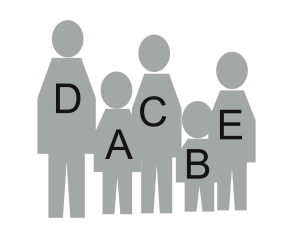
\includegraphics[scale=0.4]{uppstallning.png}
\end{minipage}

\end{figure}

Unfortunately, you could not crack the puzzle and must secretly sneak away and write a computer program that solves it.
To make it easier for yourself the next time the children challenge you, you want to be able to vary both the number of children (between 3 and 8, inclusive) and the information on the notes.
You may assume that all children have different heights and that they have not made any mistakes when writing the notes.
Interestingly, there is never more than one solution.

\section*{Input}
The first line of input consists of an integer $n$ ($3 \le n \le 8$), the number of children.

Then follow $n$ lines with two integers each: the number of children to the left who are taller than the child itself, and the number to the right.

\section*{Output}
Output a single line with $n$ characters describing the children's lineup, as a permutation of the letters \texttt{A}, \texttt{B}, \texttt{C}, etc.

\section*{Scoring}
Your solution will be tested on a set of test groups.
To earn points for a group, you must pass all test cases in that group.


\noindent
\begin{tabular}{| l | l | p{12cm} |}
  \hline
  \textbf{Group} & \textbf{Points} & \textbf{Constraints} \\ \hline
  $1$    & $20$       & $n = 3$ \\ \hline
  $2$    & $80$       & No additional constraints. \\ \hline
\end{tabular}
